% =============================================================
%  Chapter -- Converter
%  The chapter heading and introduction; one file per subsection:
%    ac-side.tex      internal voltage, modulation index, arm voltages
%                     and currents, third harmonic, limits, DC side
%    losses.tex       loss models percent_losses and detailed
%    capacitors.tex   submodule capacitor voltage ripple, inner
%                     modulation index
%    example.tex      worked example (Figure arm waveforms; Tables
%                     losses, capacitors)
%  Figures and tables: fig/, generated by fig/converter_example.py from
%  tools/example_data.py (converter at the operating point of the station
%  example, Section 4.4).
%  Sources: [1] hvdc_lf, src/hvdc_lf/components/converter, arm_reactor.
% =============================================================
\section{Converter}
\label{sec:converter}

The converter is a half-bridge MMC: three phase legs, each with an upper and a lower arm of $N$ submodules and one
arm reactor. Its input is the valve-side voltage $U_{valve}$, the active and reactive power $P_{ac}$, $Q_{ac}$ at the
valve terminals (from the transformer) and the DC voltage $U_{dc}$ across its terminals (from the DC side); its
output is the DC power, the internal voltage, the arm quantities, the losses and the limit checks. The model assumes
balanced operation without circulating current and submodules of equal capacitor voltage within an arm. The arm
reactors are a component of their own, the semiconductors as well (Section~\ref{sec:thermal}).

\subsection{Internal Voltage and Arm Quantities}
\label{sec:converter-arm}

\subsubsection{Internal voltage and modulation index}

The upper and lower arm reactors of a phase act in parallel for the AC current, so the equivalent reactance per
phase is $X = \omega \cdot L_{arm} / 2$. With the valve-side phase voltage $U_{ph} = U_{valve} / \sqrt{3}$ as phase
reference, the AC current towards the grid and the internal voltage behind the arm reactors are
\begin{equation}
  \underline{I} = \frac{\left( P_{ac} + \mathrm{j} \cdot Q_{ac} \right)^{*}}{3 \cdot U_{ph}} , \qquad
  \underline{E} = U_{ph} + \mathrm{j} \cdot X \cdot \underline{I} , \qquad
  U_{conv} = \sqrt{3} \cdot |\underline{E}| .
\end{equation}
The arm reactance carries no active power; it absorbs $Q_{arm} = 3 \cdot X \cdot I^2$. The modulation index is the
peak phase voltage in per unit of half the DC voltage:
\begin{equation}
  m = \frac{2 \cdot \sqrt{2} \cdot U_{conv}}{\sqrt{3} \cdot U_{dc}} .
\end{equation}

\subsubsection{Arm voltages and currents}

Over one period, with $e(t) = \sqrt{2} \cdot |\underline{E}| \cdot \cos(\omega t)$ and the AC current $i_{ac}(t)$,
the arms of phase a carry
\begin{align}
  u_{upper}(t) &= \frac{U_{dc}}{2} - \left( e(t) + e_3(t) \right) , &
  i_{upper}(t) &= -\frac{I_{dc}}{3} - \frac{i_{ac}(t)}{2} , \\
  u_{lower}(t) &= \frac{U_{dc}}{2} + \left( e(t) + e_3(t) \right) , &
  i_{lower}(t) &= -\frac{I_{dc}}{3} + \frac{i_{ac}(t)}{2} ,
\end{align}
with the arm currents in their physical direction (upper arm towards the positive terminal) and $I_{dc} > 0$ into
the positive terminal (inverter). Each arm carries a third of the DC current and half of the AC current:
\begin{equation}
  I_{arm\_rms} = \sqrt{\left( \frac{I_{dc}}{3} \right)^2 + \left( \frac{I_{ac}}{2} \right)^2} , \qquad
  I_{arm\_peak} = \frac{|I_{dc}|}{3} + \frac{\sqrt{2} \cdot I_{ac}}{2} .
\end{equation}
The arm reactor losses are $P_{loss\_arm} = 6 \cdot R_{arm} \cdot I_{arm\_rms}^2$. The inserted submodules of an arm
follow its voltage, $n_{ins}(t) = u_{arm}(t) / u_{sm}$, bounded by 0 and $N$.

\subsubsection{Third harmonic injection}

With third harmonic injection the arm voltages contain the zero-sequence component
$e_3(t) = -\tfrac{\sqrt{2} \cdot |\underline{E}|}{6} \cdot \cos(3 \omega t)$. It cancels between the phases and does
not change the AC side; it lowers the peak of $e + e_3$ to $\sqrt{3}/2$ of the fundamental peak. The peak factor is
$k_3 = 1$ without and $k_3 = \sqrt{3}/2$ with injection.

\subsubsection{Limits}

A half-bridge arm cannot produce a negative voltage, and its voltage cannot exceed the sum of its capacitor
voltages:
\begin{equation}
  k_3 \cdot m \le 1 , \qquad
  U_{arm\_max} = \frac{U_{dc}}{2} \cdot \left( 1 + k_3 \cdot m \right) \le N \cdot u_{sm} .
\end{equation}
The highest modulation index at a given DC voltage is therefore
$m_{max} = \min\left( 1, \, 2 \cdot N \cdot u_{sm} / U_{dc} - 1 \right) / k_3$. An exceeded limit is a warning of
the result; the calculation is not stopped. The reactive power the converter can provide at a given active power is
the circle $|\underline{E}| \le E_{max}$ in the $PQ$ plane, with centre $Q = -U_{valve}^2 / X$ and radius
$U_{valve} \cdot E_{max} / X$, $E_{max} = m_{max} \cdot \sqrt{3} \cdot U_{dc} / (2 \cdot \sqrt{2})$ line-to-line.

\subsubsection{DC side}

The DC power is the AC power plus the losses, and the DC current follows from the DC voltage:
\begin{equation}
  P_{dc} = P_{ac} + P_{loss\_cv} , \qquad I_{dc} = \frac{P_{dc}}{U_{dc}} ,
\end{equation}
both in the convention of Section~\ref{sec:conventions} ($P_{dc} < 0$ for a rectifier). The converter can also be
calculated with $P_{dc}$ or $I_{dc}$ given; then $P_{ac} = P_{dc} - P_{loss\_cv}(P_{ac})$ is iterated to a change
below $10^{-10}$ of $|P_{dc}|$.

\subsection{Losses}
\label{sec:converter-losses}

\subsubsection{Loss model \texttt{percent\_losses}}

The losses are a fixed share of the throughput plus the arm reactors:
$P_{loss\_cv} = \tfrac{p_{loss}}{100} \cdot |P_{ac}| + 6 \cdot R_{arm} \cdot I_{arm\_rms}^2$.

\subsubsection{Loss model \texttt{detailed}}

The detailed model calculates the semiconductor losses from the arm voltages and currents of one period, sampled at
$M = 360$ points. In every arm the current flows through one switch position of each submodule: through the upper
switch position (T1/D1) of an inserted submodule and through the lower switch position (T2/D2) of a bypassed one. In
the upper position the diode D1 conducts the charging current ($-i_{arm} > 0$, into the capacitor) and the IGBT T1
the discharging current; in the lower position T2 conducts the charging and D2 the discharging current. With
$n_{par}$ modules in parallel at each switch position, the current shares equally and the conduction losses of one
switch position are, with the on-state model $v = v_0 + r \cdot i$ of Section~\ref{sec:semiconductor},
\begin{equation}
  p_{cond}(i) = v_0 \cdot |i| + \frac{r \cdot i^2}{n_{par}} .
\end{equation}
The conduction losses of an arm are the mean over the period of
\begin{equation}
  n_{ins}(t) \cdot p_{ins}\!\left( i_{arm}(t) \right) + \left( N - n_{ins}(t) \right) \cdot p_{byp}\!\left( i_{arm}(t) \right) ,
\end{equation}
with $p_{ins}$ the diode (charging) or the IGBT (discharging) of the inserted position and $p_{byp}$ the IGBT
(charging) or the diode (discharging) of the bypassed position. The switching losses scale the datasheet energies
linearly with the submodule voltage and the current:
\begin{equation}
  P_{sw\_arm} = N \cdot f_{sw} \cdot \left( E_{on} + E_{off} + E_{rec} \right) \cdot \frac{u_{sm}}{U_{sw\_ref}}
                \cdot \frac{\overline{|i_{arm}|}}{I_{sw\_ref}} ,
\end{equation}
with $f_{sw}$ the average switching frequency of a submodule and $\overline{|i_{arm}|}$ the mean of the absolute arm
current. Each switching event at a switch position is shared by its $n_{par}$ modules, so $P_{sw\_arm}$ does not
depend on $n_{par}$; the slope part of the conduction losses decreases with $1/n_{par}$ and the threshold part does
not. Constant losses per submodule $p_{sm}$ (gate unit supply, capacitor, bleeder resistor) add $6 \cdot N \cdot p_{sm}$.
The converter losses are
\begin{equation}
  P_{loss\_cv} = \sum_{6\ \mathrm{arms}} \left( P_{cond\_arm} + P_{sw\_arm} \right) + 6 \cdot N \cdot p_{sm}
                 + 6 \cdot R_{arm} \cdot I_{arm\_rms}^2 .
\end{equation}
The upper and lower arms of a phase have the same losses; the three phases are equal.

\subsubsection{Loss iteration}

The arm currents contain $I_{dc} / 3$, and $I_{dc} = (P_{ac} + P_{loss\_cv}) / U_{dc}$ depends on the losses. The
losses are found by a fixed-point iteration on $P_{loss\_cv}$, starting from zero, until the change is below
$10^{-12} \cdot \max(1, |P_{ac}|)$.

\subsection{Submodule Capacitors}
\label{sec:converter-capacitors}

\subsubsection{Capacitor voltage ripple}

With the submodule capacitance $C_{sm}$ given, the variation of the capacitor voltages over one period is calculated.
An arm takes the power $p(t) = -u_{arm}(t) \cdot i_{arm}(t)$ (charging current). Its mean is the share of the
losses of the arm; the remainder charges and discharges the inserted capacitors. The energy variation of an arm is
\begin{equation}
  \Delta W(t) = \int_0^t \left( p(t') - \overline{p} \right) \mathrm{d}t' ,
\end{equation}
evaluated over the $M$ samples. Around the stored energy $W_0 = N \cdot C_{sm} \cdot u_{sm}^2 / 2$ of an arm,
with the capacitors of an arm balanced and $u_{sm}$ their average voltage,
\begin{equation}
  W(t) = W_0 + \Delta W(t) - \overline{\Delta W} , \qquad
  u_c(t) = \sqrt{\frac{2 \cdot W(t)}{N \cdot C_{sm}}} .
\end{equation}
The result gives the stored energy of the six arms, per MV$\cdot$A of $|\underline{S}_{ac}|$, the peak-to-peak
energy variation of an arm, the lowest and highest capacitor voltage and the ripple in per cent of $u_{sm}$. The
ripple does not change $P$ and $Q$ of the load flow. A capacitance so small that $W(t) \le 0$ is rejected.

\subsubsection{Inner modulation index}

The inner modulation index relates the voltage an arm produces to the sum of its capacitor voltages:
\begin{equation}
  a = \max_t \frac{u_{arm}(t)}{N \cdot u_c(t)} \le 1 ,
\end{equation}
with $u_c = u_{sm}$ when no capacitance is given, $a = U_{arm\_max} / (N \cdot u_{sm})$. The margin
$\min_t \left( N \cdot u_c(t) - u_{arm}(t) \right)$ is the voltage reserve of the arm; $a > 1$ is a warning. The
capacitor ripple shifts $a$ in either direction: $a$ rises if the capacitors of an arm are below average when the
arm voltage is highest and falls if they are above average, depending on the operating point.

\subsection{Worked Example}
\label{sec:converter-example}

The converter of the example station at its operating point of Section~\ref{sec:station-example} has
$U_{valve} = \cvUv$\,kV, $P_{ac} = \cvP$\,MW, $Q_{ac} = \cvQ$\,Mvar and $U_{dc} = \cvUdc$\,kV. The arm
currents are $I_{arm\_rms} = \cvIrms$\,kA and $I_{arm\_peak} = \cvIpk$\,kA. Figure~\ref{fig:converter-arm} shows the arm voltages,
the arm currents and the capacitor voltages of phase a over one period; Table~\ref{tab:converter-losses} gives the
losses of the detailed model and Table~\ref{tab:converter-capacitors} the capacitor quantities.

\begin{figure}[!ht]
  \centering
  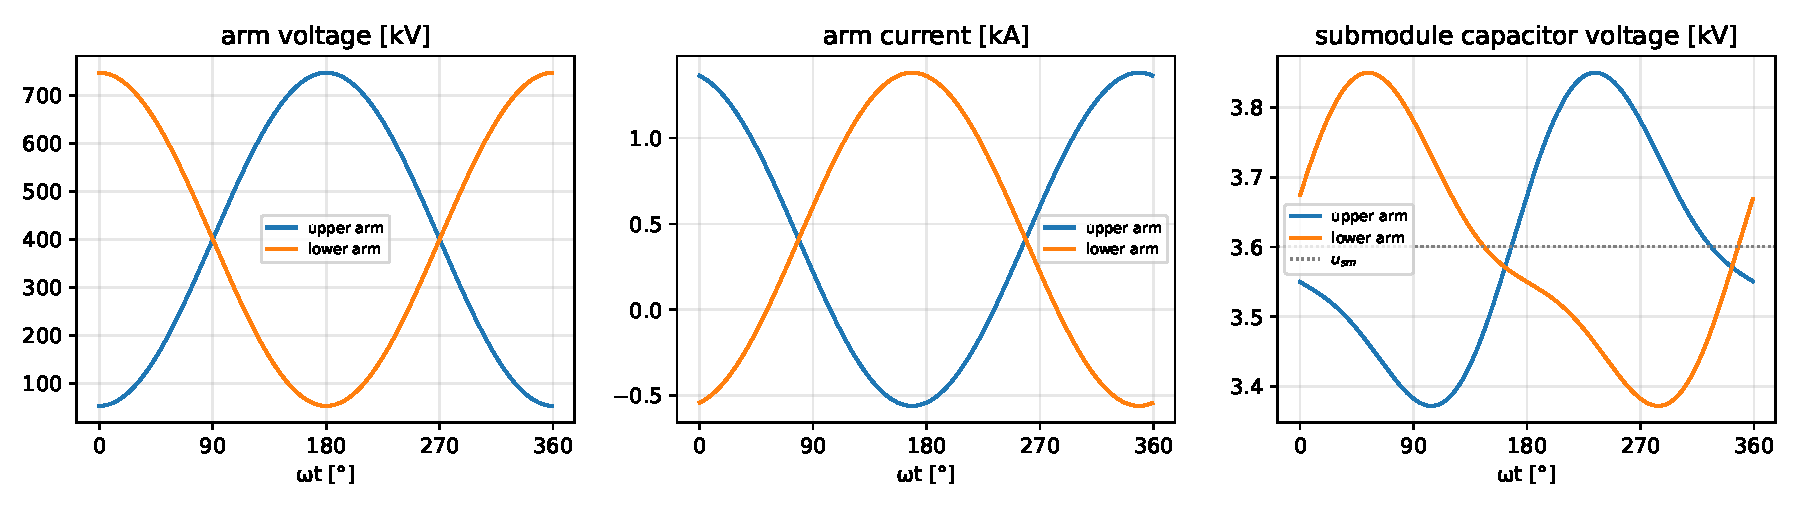
\includegraphics[width=\linewidth]{converter/fig/arm_waveforms.pdf}
  \caption{Arm voltages, arm currents and submodule capacitor voltages of phase a over one period, converter of the
           example at $P_{ac} = \cvP$\,MW (rectifier)}
  \label{fig:converter-arm}
\end{figure}

\begin{table}[!ht]
  \centering
  \small
  \begin{tabular}{@{}l r r@{}}
    \toprule
    \textbf{Part} & \multicolumn{1}{c}{\textbf{MW}} & \multicolumn{1}{c}{\textbf{\% of $|P_{ac}|$}} \\
    \midrule
    \tablerows{converter/fig/losses_table}
    \bottomrule
  \end{tabular}
  \caption{Converter losses of the example, loss model \texttt{detailed}, two modules in parallel}
  \label{tab:converter-losses}
\end{table}

\begin{table}[!ht]
  \centering
  \small
  \begin{tabular}{@{}l r l@{}}
    \toprule
    \textbf{Quantity} & \multicolumn{1}{c}{\textbf{Value}} & \multicolumn{1}{c}{\textbf{Unit}} \\
    \midrule
    \tablerows{converter/fig/capacitor_table}
    \bottomrule
  \end{tabular}
  \caption{Modulation and submodule capacitor quantities of the example, $C_{sm} = 3.7$\,mF}
  \label{tab:converter-capacitors}
\end{table}
\FloatBarrier

